\documentclass[]{article}
\usepackage{lmodern}
\usepackage{amssymb,amsmath}
\usepackage{ifxetex,ifluatex}
\usepackage{fixltx2e} % provides \textsubscript
\ifnum 0\ifxetex 1\fi\ifluatex 1\fi=0 % if pdftex
  \usepackage[T1]{fontenc}
  \usepackage[utf8]{inputenc}
\else % if luatex or xelatex
  \ifxetex
    \usepackage{mathspec}
  \else
    \usepackage{fontspec}
  \fi
  \defaultfontfeatures{Ligatures=TeX,Scale=MatchLowercase}
\fi
% use upquote if available, for straight quotes in verbatim environments
\IfFileExists{upquote.sty}{\usepackage{upquote}}{}
% use microtype if available
\IfFileExists{microtype.sty}{%
\usepackage{microtype}
\UseMicrotypeSet[protrusion]{basicmath} % disable protrusion for tt fonts
}{}
\usepackage[margin=1in]{geometry}
\usepackage{hyperref}
\hypersetup{unicode=true,
            pdftitle={Satellite field verification results},
            pdfauthor={KBG},
            pdfborder={0 0 0},
            breaklinks=true}
\urlstyle{same}  % don't use monospace font for urls
\usepackage{longtable,booktabs}
\usepackage{graphicx,grffile}
\makeatletter
\def\maxwidth{\ifdim\Gin@nat@width>\linewidth\linewidth\else\Gin@nat@width\fi}
\def\maxheight{\ifdim\Gin@nat@height>\textheight\textheight\else\Gin@nat@height\fi}
\makeatother
% Scale images if necessary, so that they will not overflow the page
% margins by default, and it is still possible to overwrite the defaults
% using explicit options in \includegraphics[width, height, ...]{}
\setkeys{Gin}{width=\maxwidth,height=\maxheight,keepaspectratio}
\IfFileExists{parskip.sty}{%
\usepackage{parskip}
}{% else
\setlength{\parindent}{0pt}
\setlength{\parskip}{6pt plus 2pt minus 1pt}
}
\setlength{\emergencystretch}{3em}  % prevent overfull lines
\providecommand{\tightlist}{%
  \setlength{\itemsep}{0pt}\setlength{\parskip}{0pt}}
\setcounter{secnumdepth}{0}
% Redefines (sub)paragraphs to behave more like sections
\ifx\paragraph\undefined\else
\let\oldparagraph\paragraph
\renewcommand{\paragraph}[1]{\oldparagraph{#1}\mbox{}}
\fi
\ifx\subparagraph\undefined\else
\let\oldsubparagraph\subparagraph
\renewcommand{\subparagraph}[1]{\oldsubparagraph{#1}\mbox{}}
\fi

%%% Use protect on footnotes to avoid problems with footnotes in titles
\let\rmarkdownfootnote\footnote%
\def\footnote{\protect\rmarkdownfootnote}

%%% Change title format to be more compact
\usepackage{titling}

% Create subtitle command for use in maketitle
\newcommand{\subtitle}[1]{
  \posttitle{
    \begin{center}\large#1\end{center}
    }
}

\setlength{\droptitle}{-2em}

  \title{Satellite field verification results}
    \pretitle{\vspace{\droptitle}\centering\huge}
  \posttitle{\par}
    \author{KBG}
    \preauthor{\centering\large\emph}
  \postauthor{\par}
      \predate{\centering\large\emph}
  \postdate{\par}
    \date{December 6, 2019}


\begin{document}
\maketitle

\hypertarget{introduction}{%
\subsection{\texorpdfstring{\textbf{Introduction}}{Introduction}}\label{introduction}}

To better understand the performance of the satellite tool field
verification sampling was conducted in 2019. The tool was developed by
the San Francisco Estuary Institute (SFEI), NOAA, and the California
State Water Resources Control Boards,

This document describes the field verification procedure and presents
the initial data.

\hypertarget{methods}{%
\subsection{\texorpdfstring{\textbf{Methods}}{Methods}}\label{methods}}

\hypertarget{field-sampling}{%
\paragraph{\texorpdfstring{\emph{Field
sampling}}{Field sampling}}\label{field-sampling}}

Field sampling occurred on the same day as the Sentinel-3B flyover. In a
waterbody three pixels were selected for sampling. Within a pixel three
samples were collected, for a total of nine measurement sites (Fig. 1).
At each sampling point, a Malvern Panalytical Fielspec Handheld2 Pro
radiometer was used to collect radiance data. Each reading involved
collecting ten measurements at 1 nm wavelength resolution from 300-900
nms, which were then averaged into a single value per nm for the
reading. Readings were taken on a calibrated 10\% Spectralon reflectance
plate, the water, and the sky. All readings were taken 40-45 degrees
altitude and 115-130 degrees alzimuth from the sun. Triplicate plate,
water, and sky readings were collected at eash sampling site.

Seven sampling events occurred at four different waterbodies from August
1 to October 8, 2019 (Table 1). Only Clear Lake had satellite pixels
with positive CItotal values on the sampling days. There had been blooms
at San Pablo Reservoir and Lake San Antonio, but they had dissipated to
non-detects on the satellite by the time we were able to sample them.
Lake Almanor was chosen due to it's higher elevation and previous
questionable CItotal values generated by Meris imagery.

\begin{center}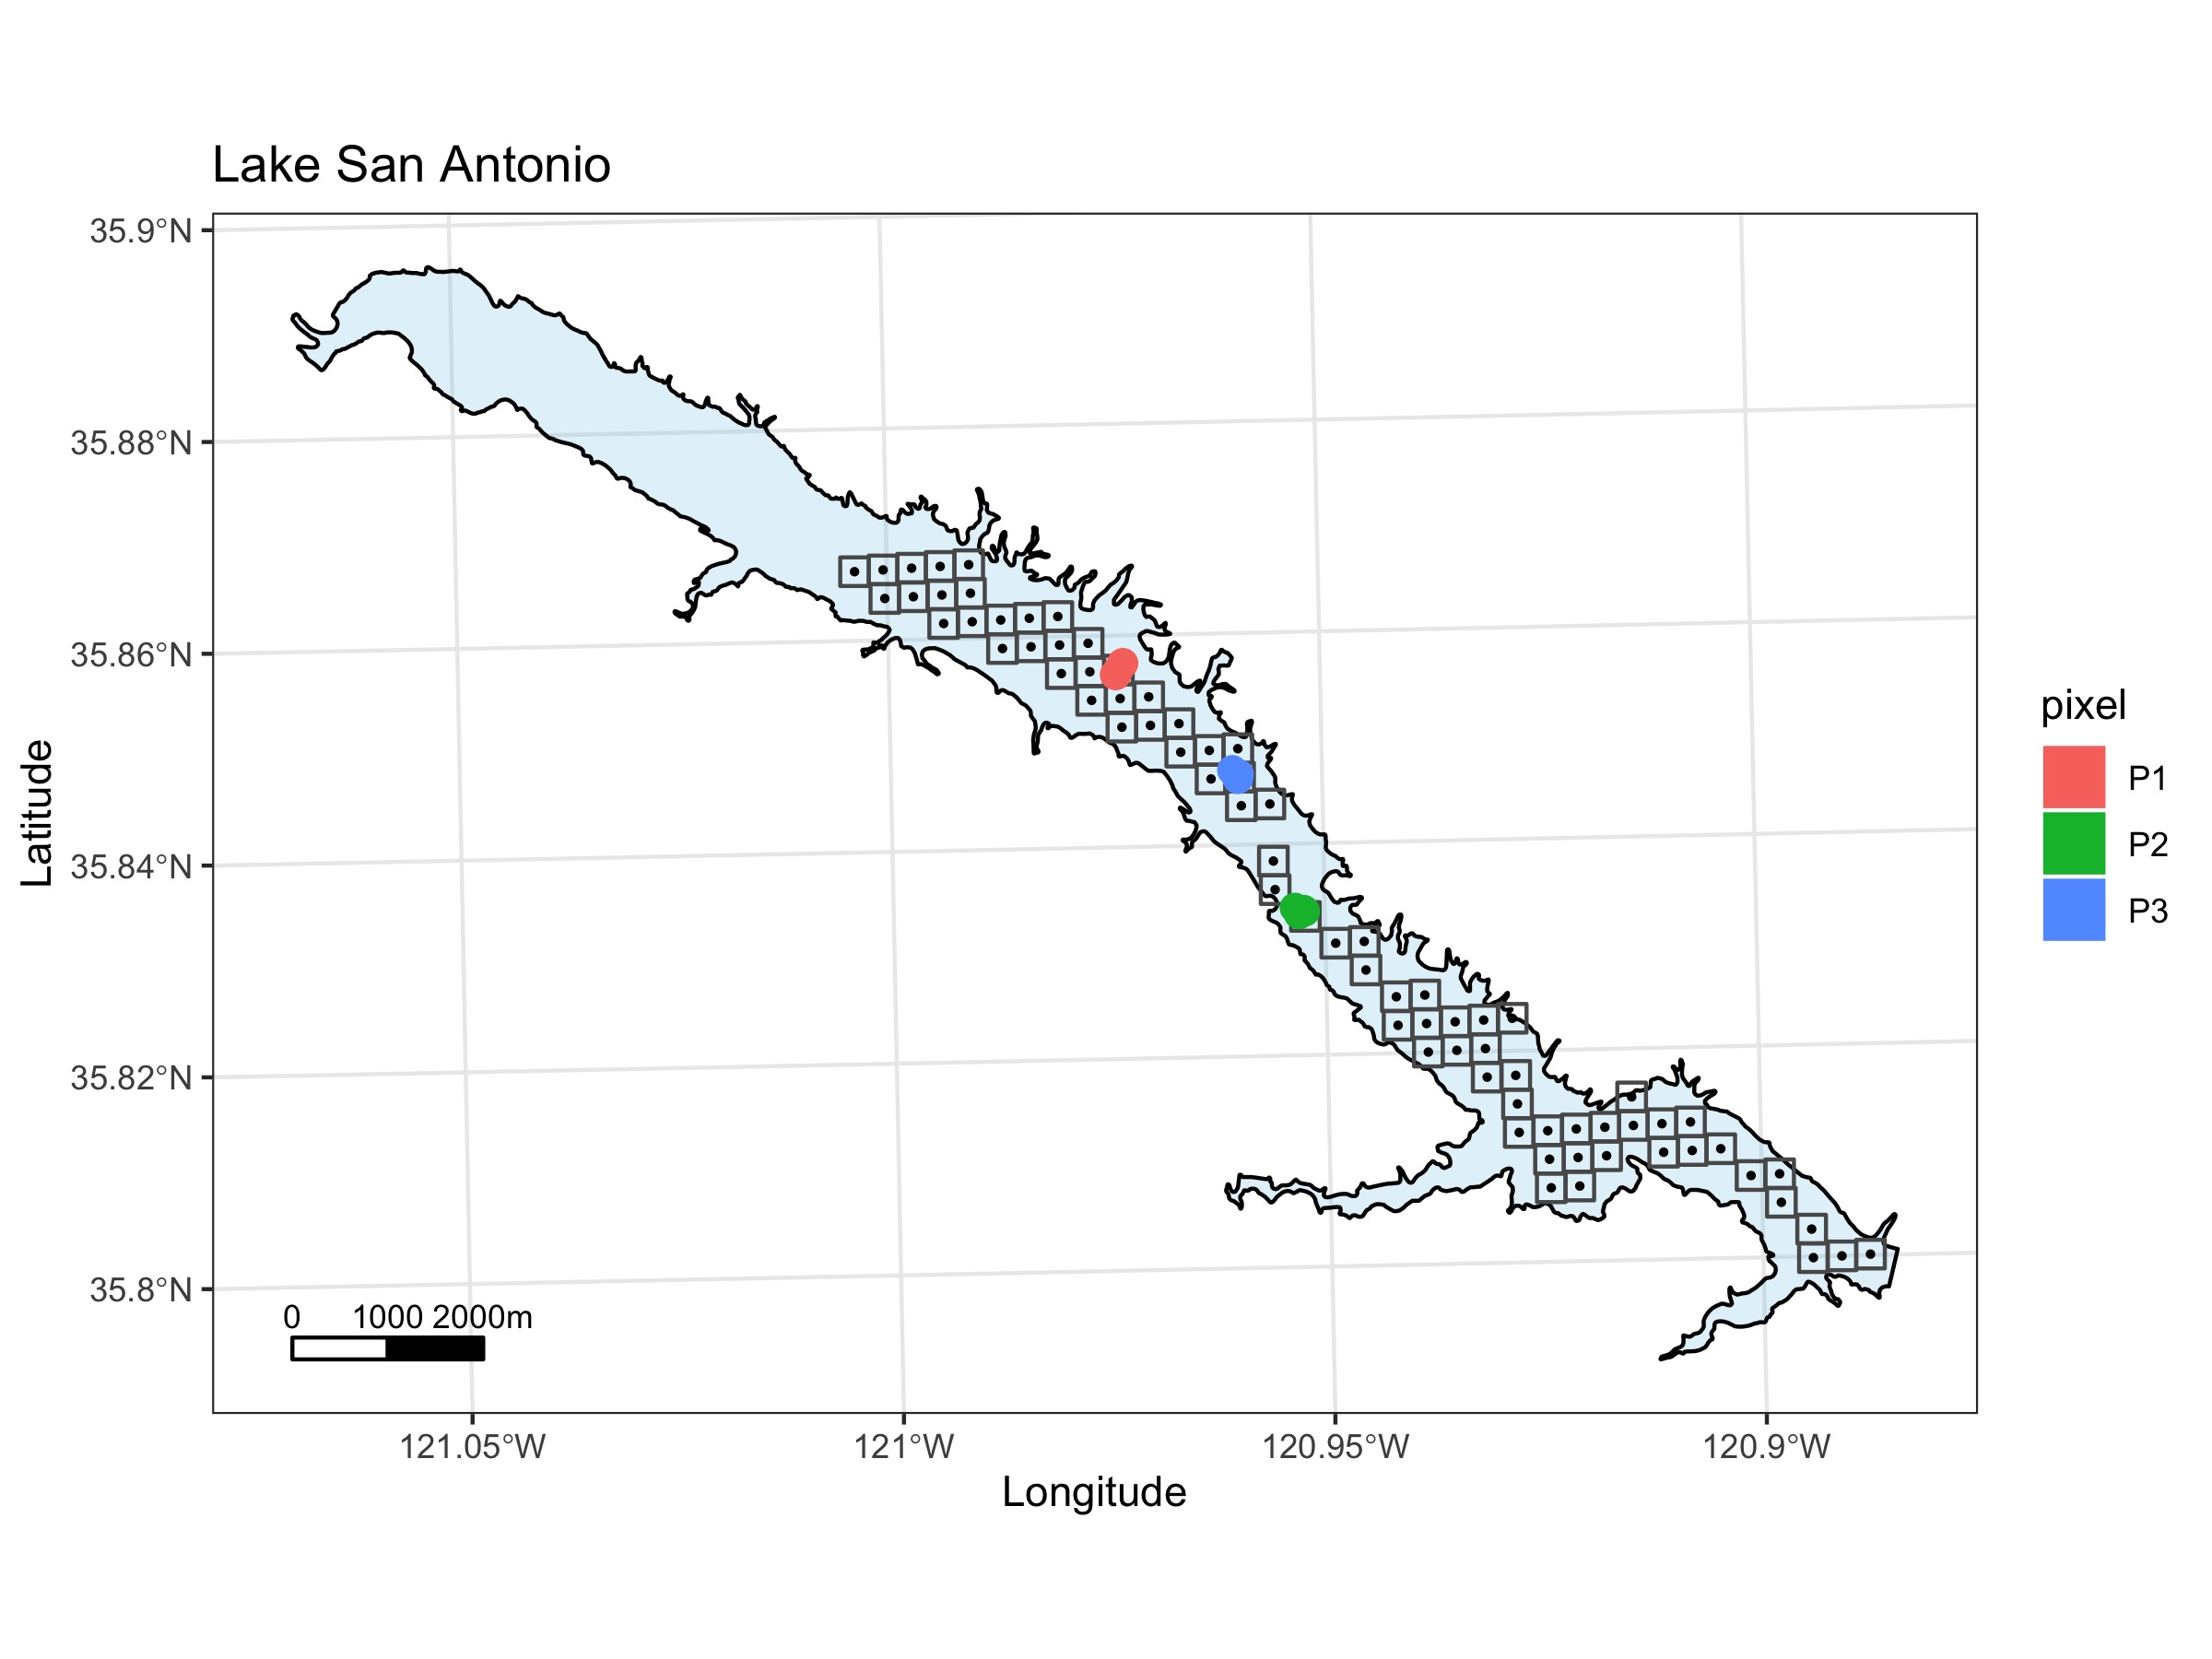
\includegraphics[width=0.3\linewidth]{../Data/20190801_LakeSanAntonio/lsa_lake_map} \end{center}

\begin{center}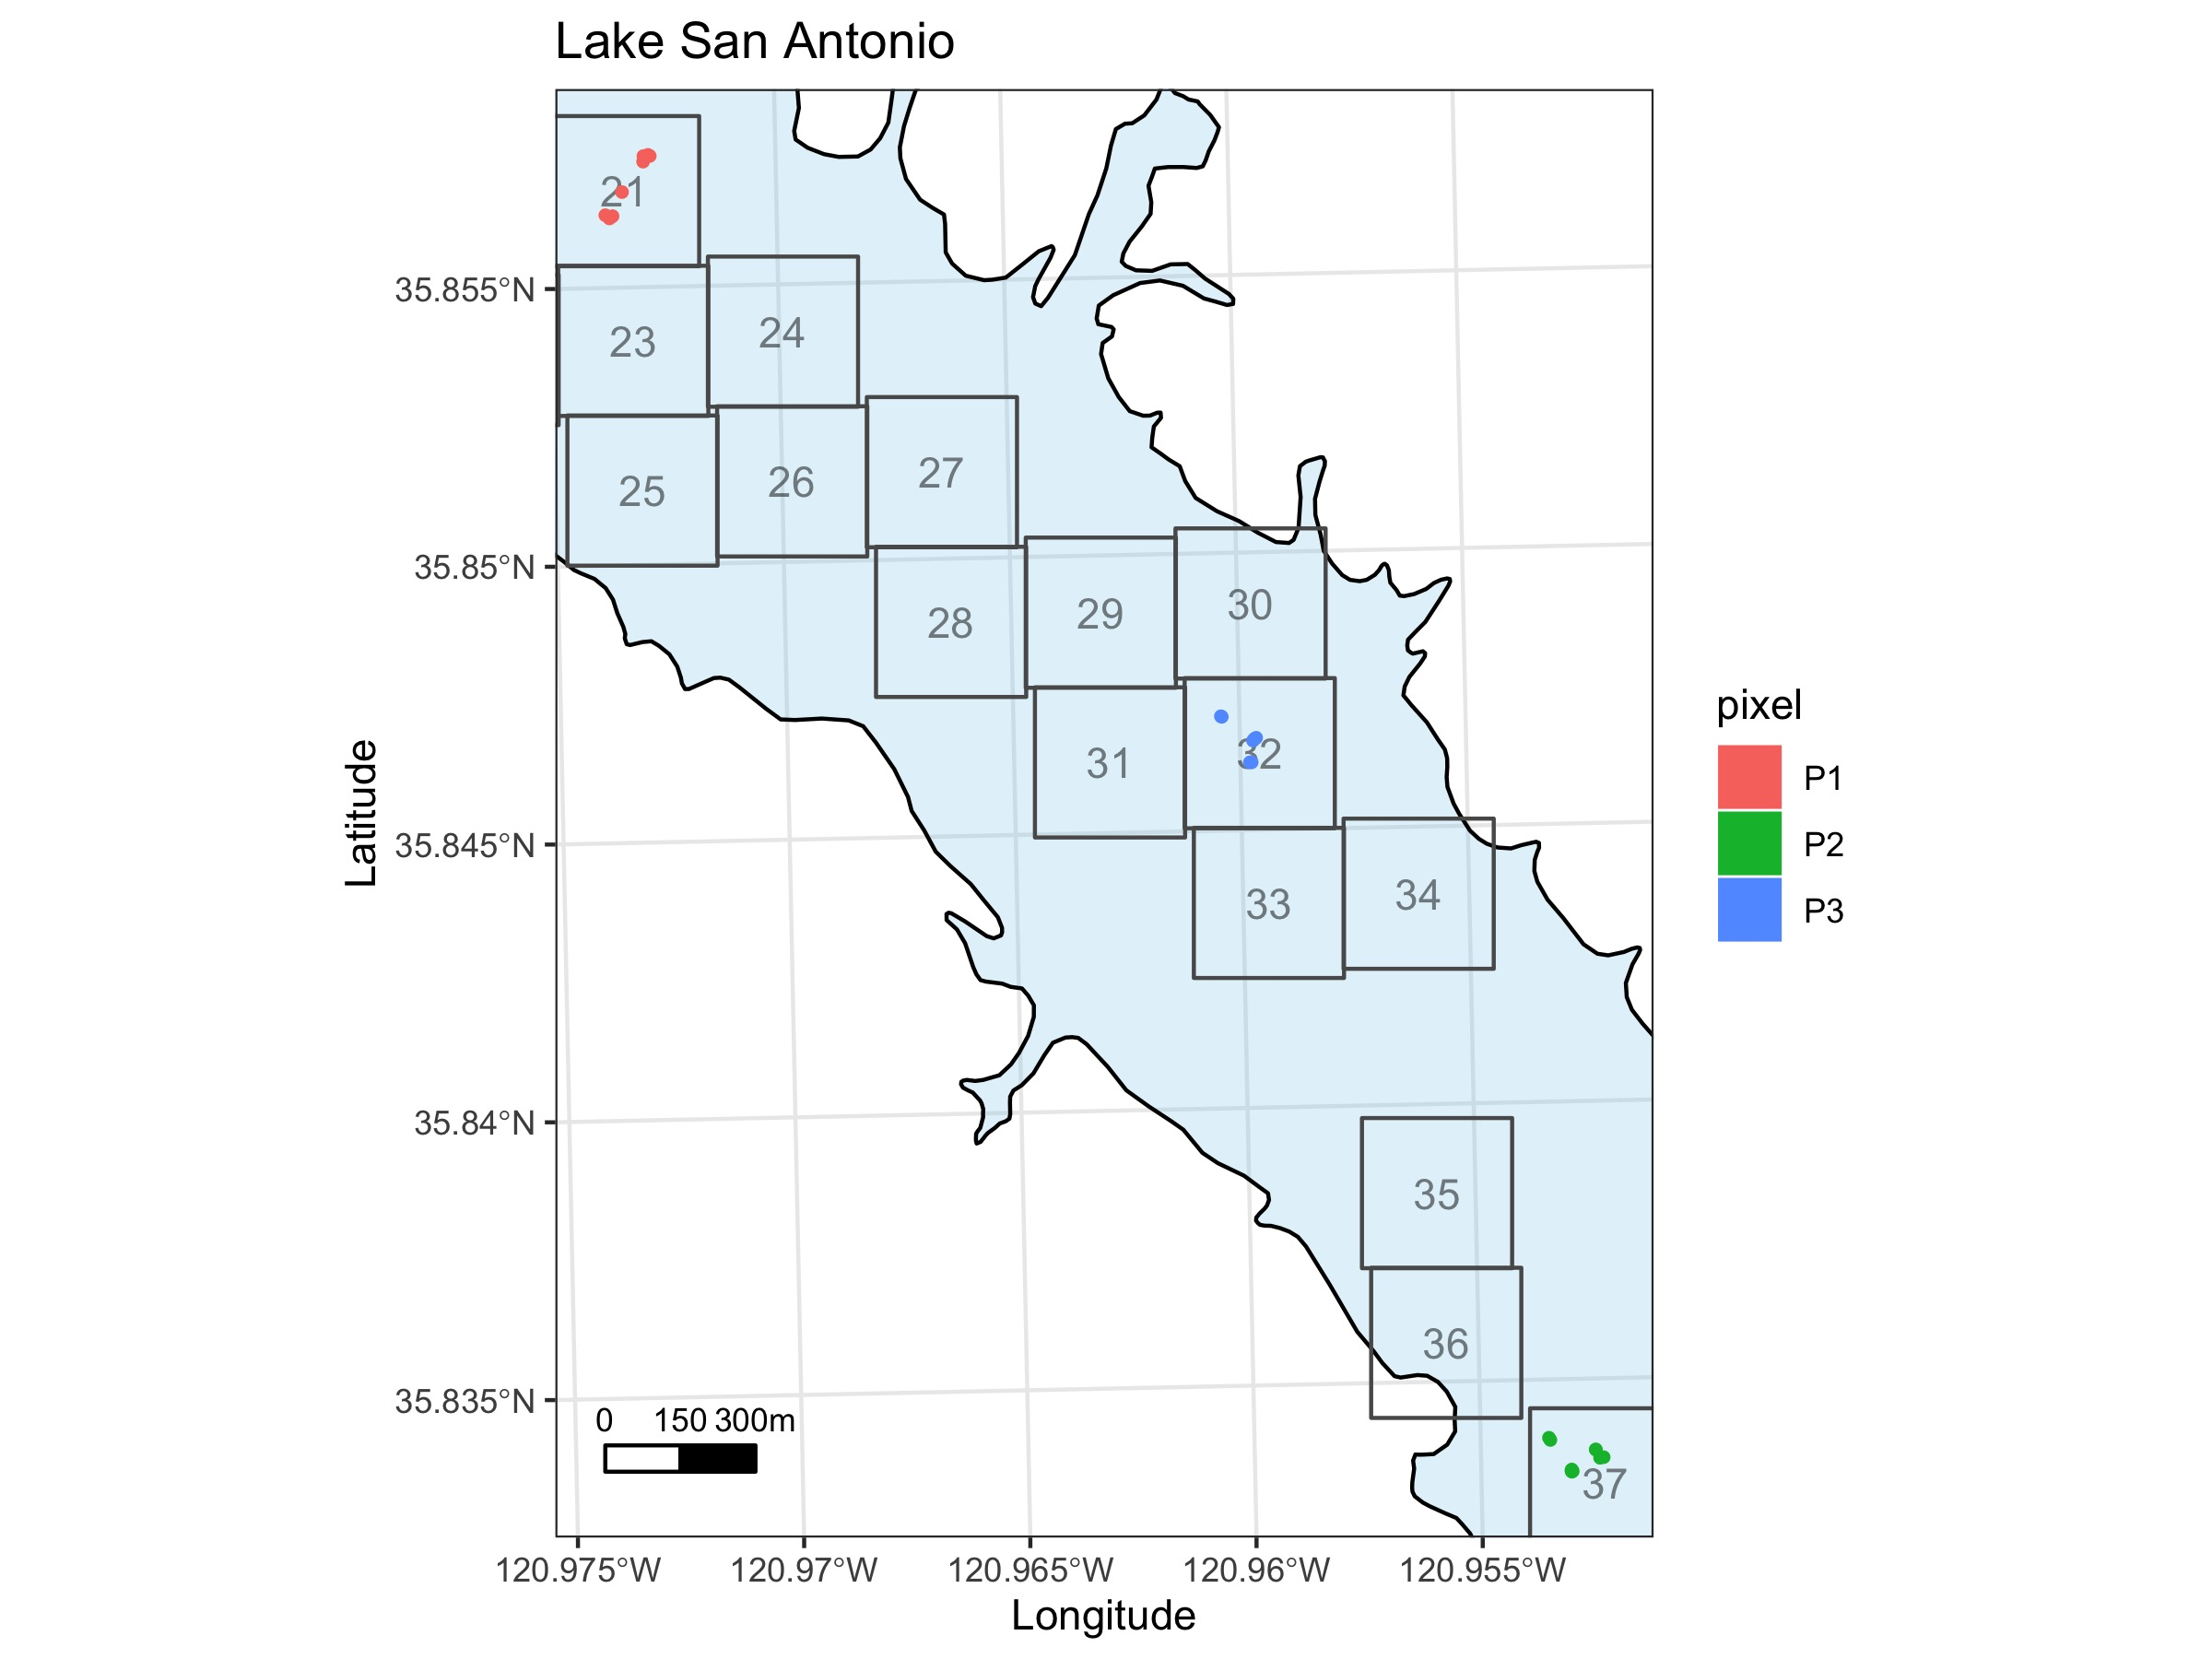
\includegraphics[width=0.3\linewidth]{../Data/20190801_LakeSanAntonio/lsa_lake_bbox_map} \end{center}

\textbf{Figure 1.} Sampling maps of Lake San Antonio. Left panel) Entire
lake showing the pixel locations for satellite imagery. Colors show the
locations of the sampling pixels. Right panel) Zoom in of the sampling
area showing the three different sampling sites within each of the three
pixels. Numbers are the pixel ID for the satellite.

\begin{longtable}[]{@{}lllll@{}}
\caption{Table 1. Waterbody information}\tabularnewline
\toprule
Name & County & Sampling.date & Size & elevation\tabularnewline
\midrule
\endfirsthead
\toprule
Name & County & Sampling.date & Size & elevation\tabularnewline
\midrule
\endhead
Clear Lake & Lake & Aug-7, Aug-16, Oct-8 & xx & xx\tabularnewline
Lake Almanor & Plumas & Aug-15 & XX & XX\tabularnewline
Lake San Antonio & Monterrey & Aug-1 & xx & xx\tabularnewline
San Pablo Reservoir & Contra Costa & Aug-12 & xx & xx\tabularnewline
\bottomrule
\end{longtable}

\hypertarget{field-radiometer-calculations}{%
\paragraph{\texorpdfstring{\emph{Field radiometer
calculations}}{Field radiometer calculations}}\label{field-radiometer-calculations}}

The raw radiance values from the radiometer were converted to remote
sensed reflectance (rrs) values per nm using the program
\texttt{test\_asd\_group.exe} provided to the Waterboards by NOAA staff.

The rrs values were then used to calculate the cyanobacterial indices CI
and CIcyano. The CI value is derived from the spectral shape at 665 nm
is calculated from equation 1 in Wynne et al.~2008:
\[SS(681) = rrs681 - rrs665 - (rrs709 - rrs665) * \frac{681-665}{709-665}]\]
More negative CI values represent higher cyanobacterial abundances in
the surface waters of a pixel. To transform into a more intuitive value
the SS(681) is converted to CI by: \[CI = -1*SS(681)\] CI values
\textless0 indicate no cyanobacteria present. However, certain water
conditions can generate positive CI values when there are no
cyanobacteria present. To reduce the frequency of false positives,
Lunetta et al.~2015 proposed an additional indice, CIcyano, based on the
spectral shape at 665 nm, which is calculated by:
\[CIcyano = rrs665 - rrs620 + (rrs620 - rrs681) * \frac{665-620}{681-620}\]

When CIcyano is \textgreater0 it indicates cyanobacteria present in the
water and when it is \textless0, cyanobacteria is predicted to be
absent. CIcyano is then transformed into a binary value of 0 when
CIcyano \textless0 and 1 when CIcyano \textgreater{} 0. Then for a given
pixel the final CI value is calculated by: \[CIfinal = CIcyano * CI\]

This will render all measurements with CIcyano = 0 as non-detects, even
if they had a positiv CI value.

\hypertarget{satellite-data-calculations}{%
\paragraph{\texorpdfstring{\emph{Satellite data
calculations}}{Satellite data calculations}}\label{satellite-data-calculations}}

Satellite data is provided from NOAA and given as an integer for each
pixel ranging in values 0-250, corresponding to increasing CIfinal
value. The pixel integer is converted to CIfinal with:
\[CI_final = 10^{0.012 * PixInteger - 4.2} \]

SFEI and the CA Waterboards then multiply CI\_final by a constant to
make the values easier to work with by putting them on a scale of
0-1000. This index is called CI\_mod and calculateted by:
\[CImod = CIfinal * 15805.18\]

\hypertarget{results}{%
\subsection{\texorpdfstring{\textbf{Results}}{Results}}\label{results}}

\hypertarget{lake-conditions}{%
\paragraph{\texorpdfstring{\emph{Lake
conditions}}{Lake conditions}}\label{lake-conditions}}

Lakes ranged in phytoplankton concentrations, with median chl-a
concentrations ranging from 1-40 ug/L (Fig. 1) and Secchi depths ranged
from \textless1 - 4.5 meters (Fig. 2). Only in Clear Lake were
cyanobacterial colonies visible, however, microscopic analysis of
samples did identify cyanobacterial taxa in some waterbodies, including
\emph{Dolichospermum}, \emph{Microcystis}, and \emph{Gloeotrichia}.

\begin{figure}

{\centering 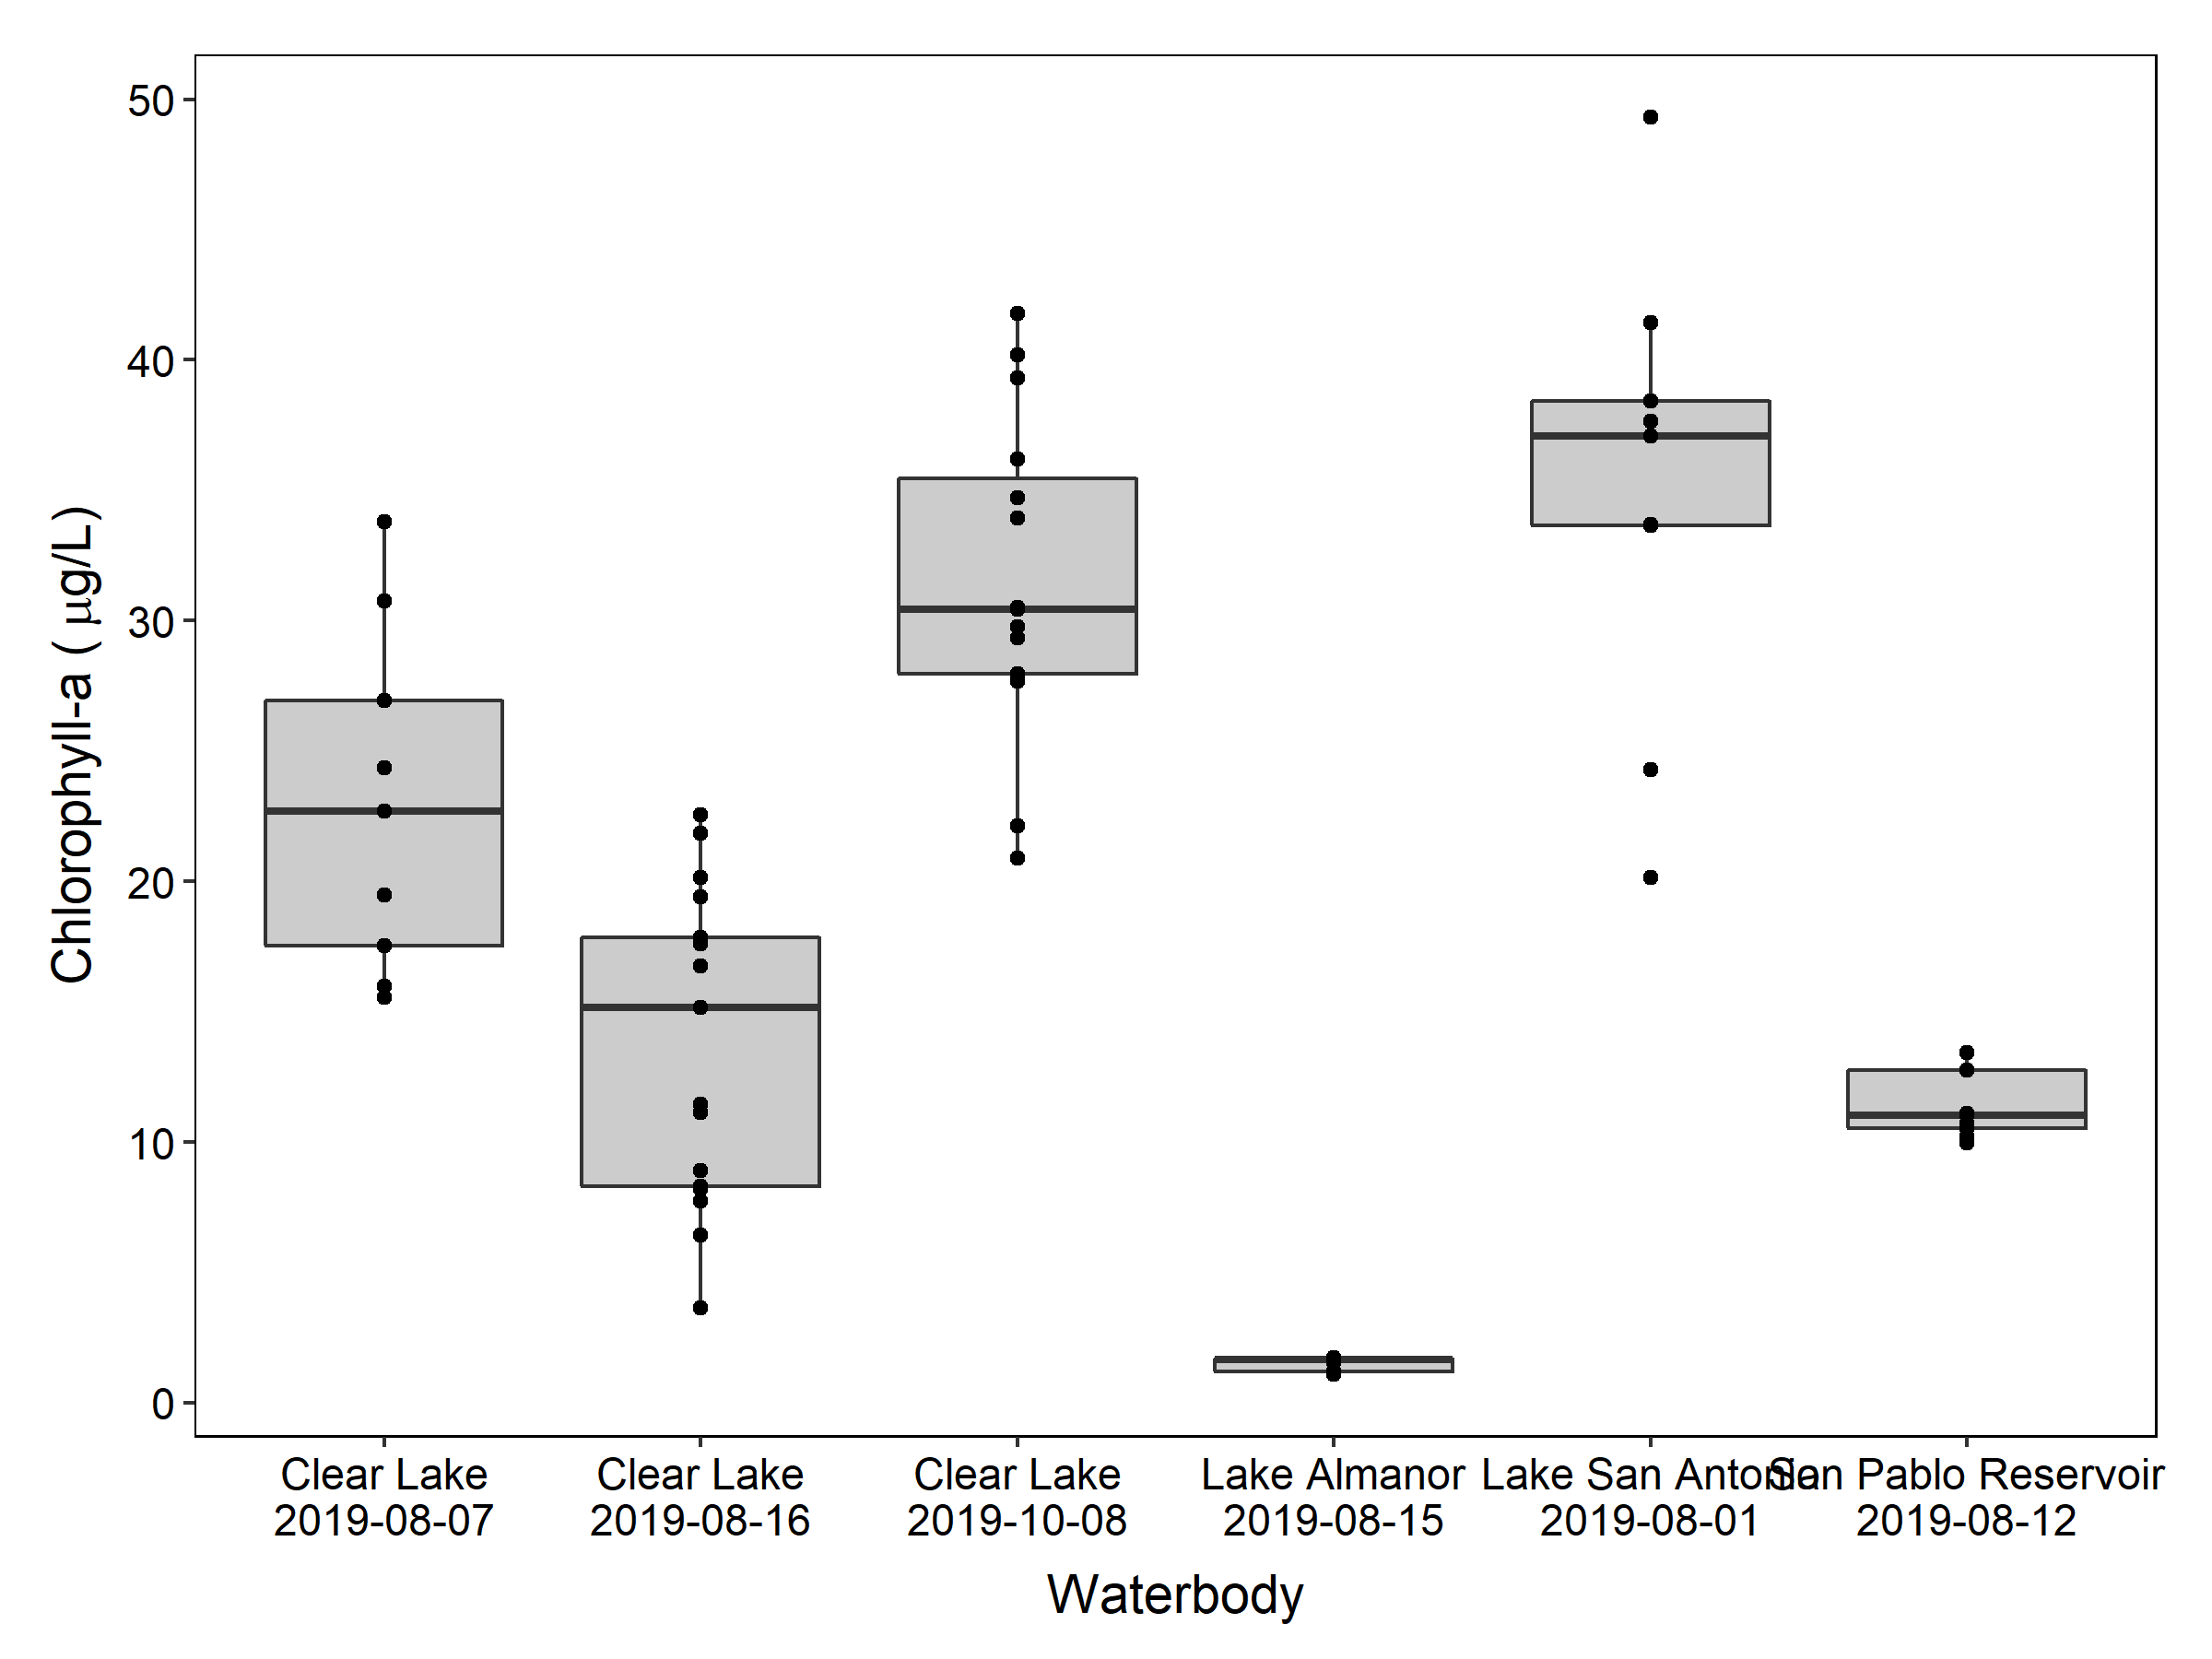
\includegraphics[width=0.6\linewidth]{../Data/Figures_output/chla} 

}

\end{figure}

\textbf{Figure 2.} Chlorophyll-a concentrations at sampling locations in
waterbodies. (Note: data is missing for Clear Lake on Aug-16 and Oct-8).

\begin{figure}

{\centering 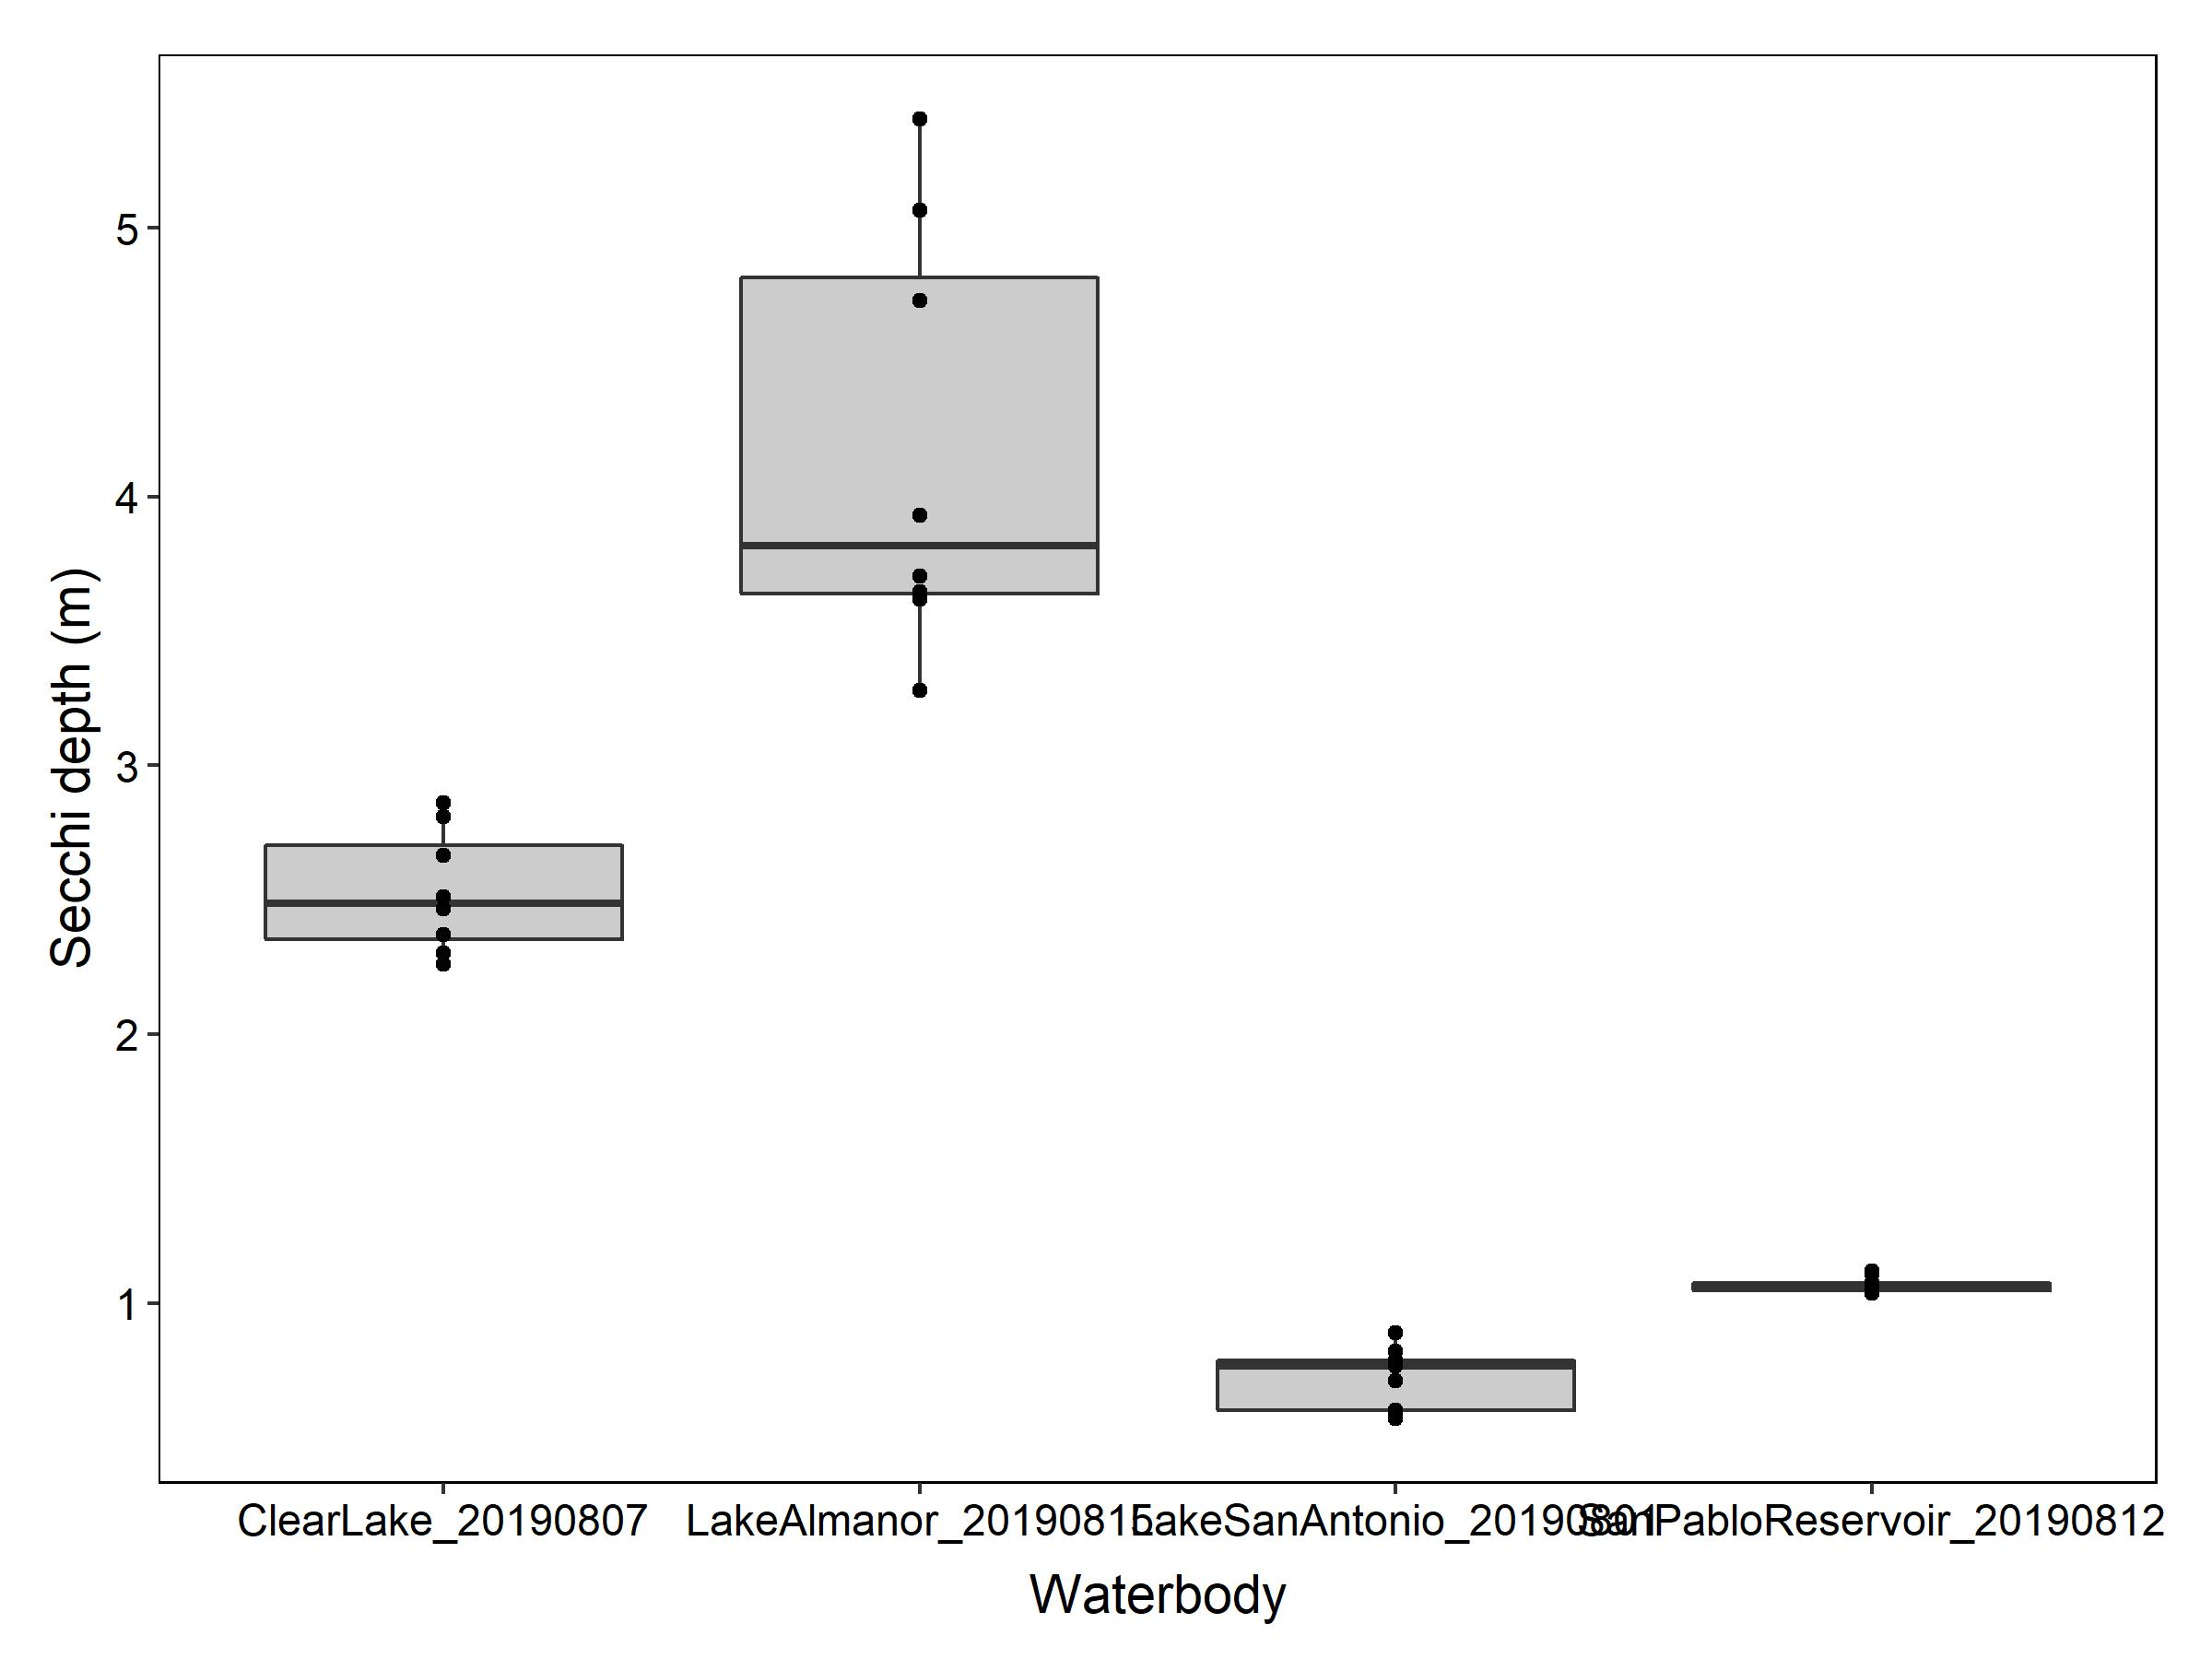
\includegraphics[width=0.6\linewidth]{../Data/Figures_output/secchi} 

}

\end{figure}

\textbf{Figure 3.} Secchi depth at sampling locations in waterbodies.
(Note: data is missing for Clear Lake on Aug-16 and Oct-8).

\begin{longtable}[]{@{}lll@{}}
\caption{Table 2. Microscopic cyanobacteria
identification.}\tabularnewline
\toprule
Name & Sampling\_date & Cyanobacteria\tabularnewline
\midrule
\endfirsthead
\toprule
Name & Sampling\_date & Cyanobacteria\tabularnewline
\midrule
\endhead
Clear Lake & Aug-7 & Microcystis, Gloeotrichia,
Dolichospermum\tabularnewline
Clear Lake & Aug-16 & No data\tabularnewline
Clear Lake & Oct-8 & No data\tabularnewline
Lake Almanor & Aug-15 & None\tabularnewline
Lake San Antonio & Aug-1 & Dolichospermum\tabularnewline
San Pablo Reservoir & Aug-12 & Dolichospermum\tabularnewline
\bottomrule
\end{longtable}

\hypertarget{cicyano-values}{%
\paragraph{\texorpdfstring{\emph{CIcyano
values}}{CIcyano values}}\label{cicyano-values}}

All 142 field CIcyano values were \textless0 suggesing that
cyanobacteria were not present at any of the field sampling locations
(Fig. 4). The range of SS(665) values was -0.0025 to -0.000071.

\begin{figure}
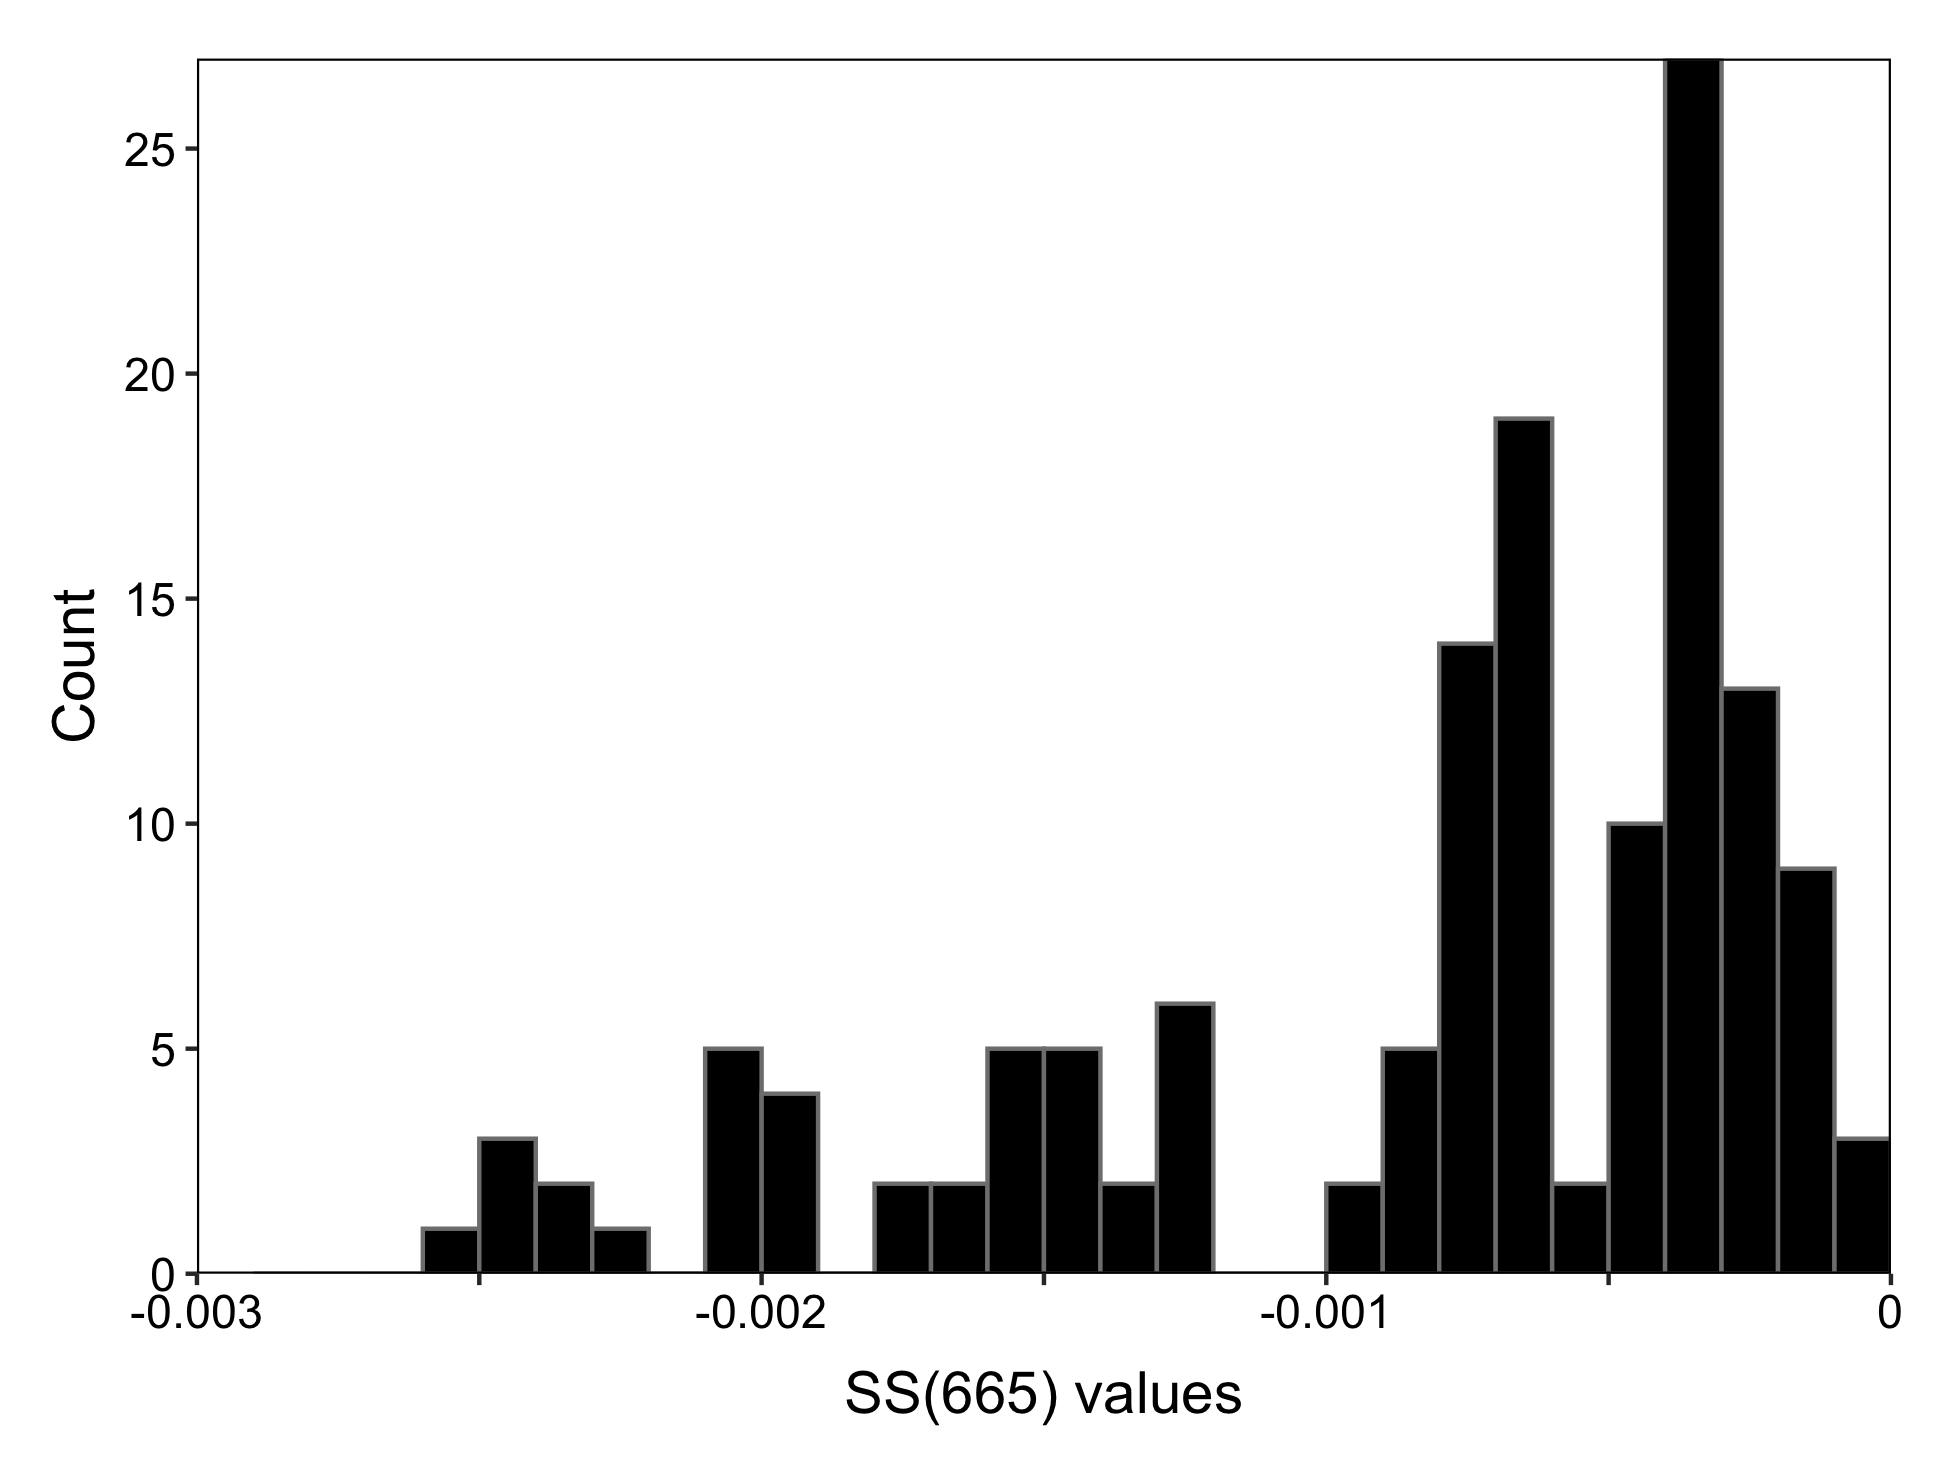
\includegraphics[width=33.33in]{../Data/Figures_output/ss665_hist} \end{figure}

\textbf{Figure 4.} Histogram of all SS(665) values (N = 142).

\hypertarget{ci-values}{%
\paragraph{\texorpdfstring{\emph{CI
values}}{CI values}}\label{ci-values}}

CIfinal values would all be zero, because all CIcyano values were
\textless0. Therefore, only the CI values will be shown in the results.
Variance among the triplicate measurements within a sample was low (Fig.
5). Lake Almanor and San Pablo reservoir had CI values \textless0
suggesting no cyanobacteria present in the waterbody. All other
waterbodies had positive CI values, suggesting the presence of
cyanobacteria.

\begin{figure}

{\centering 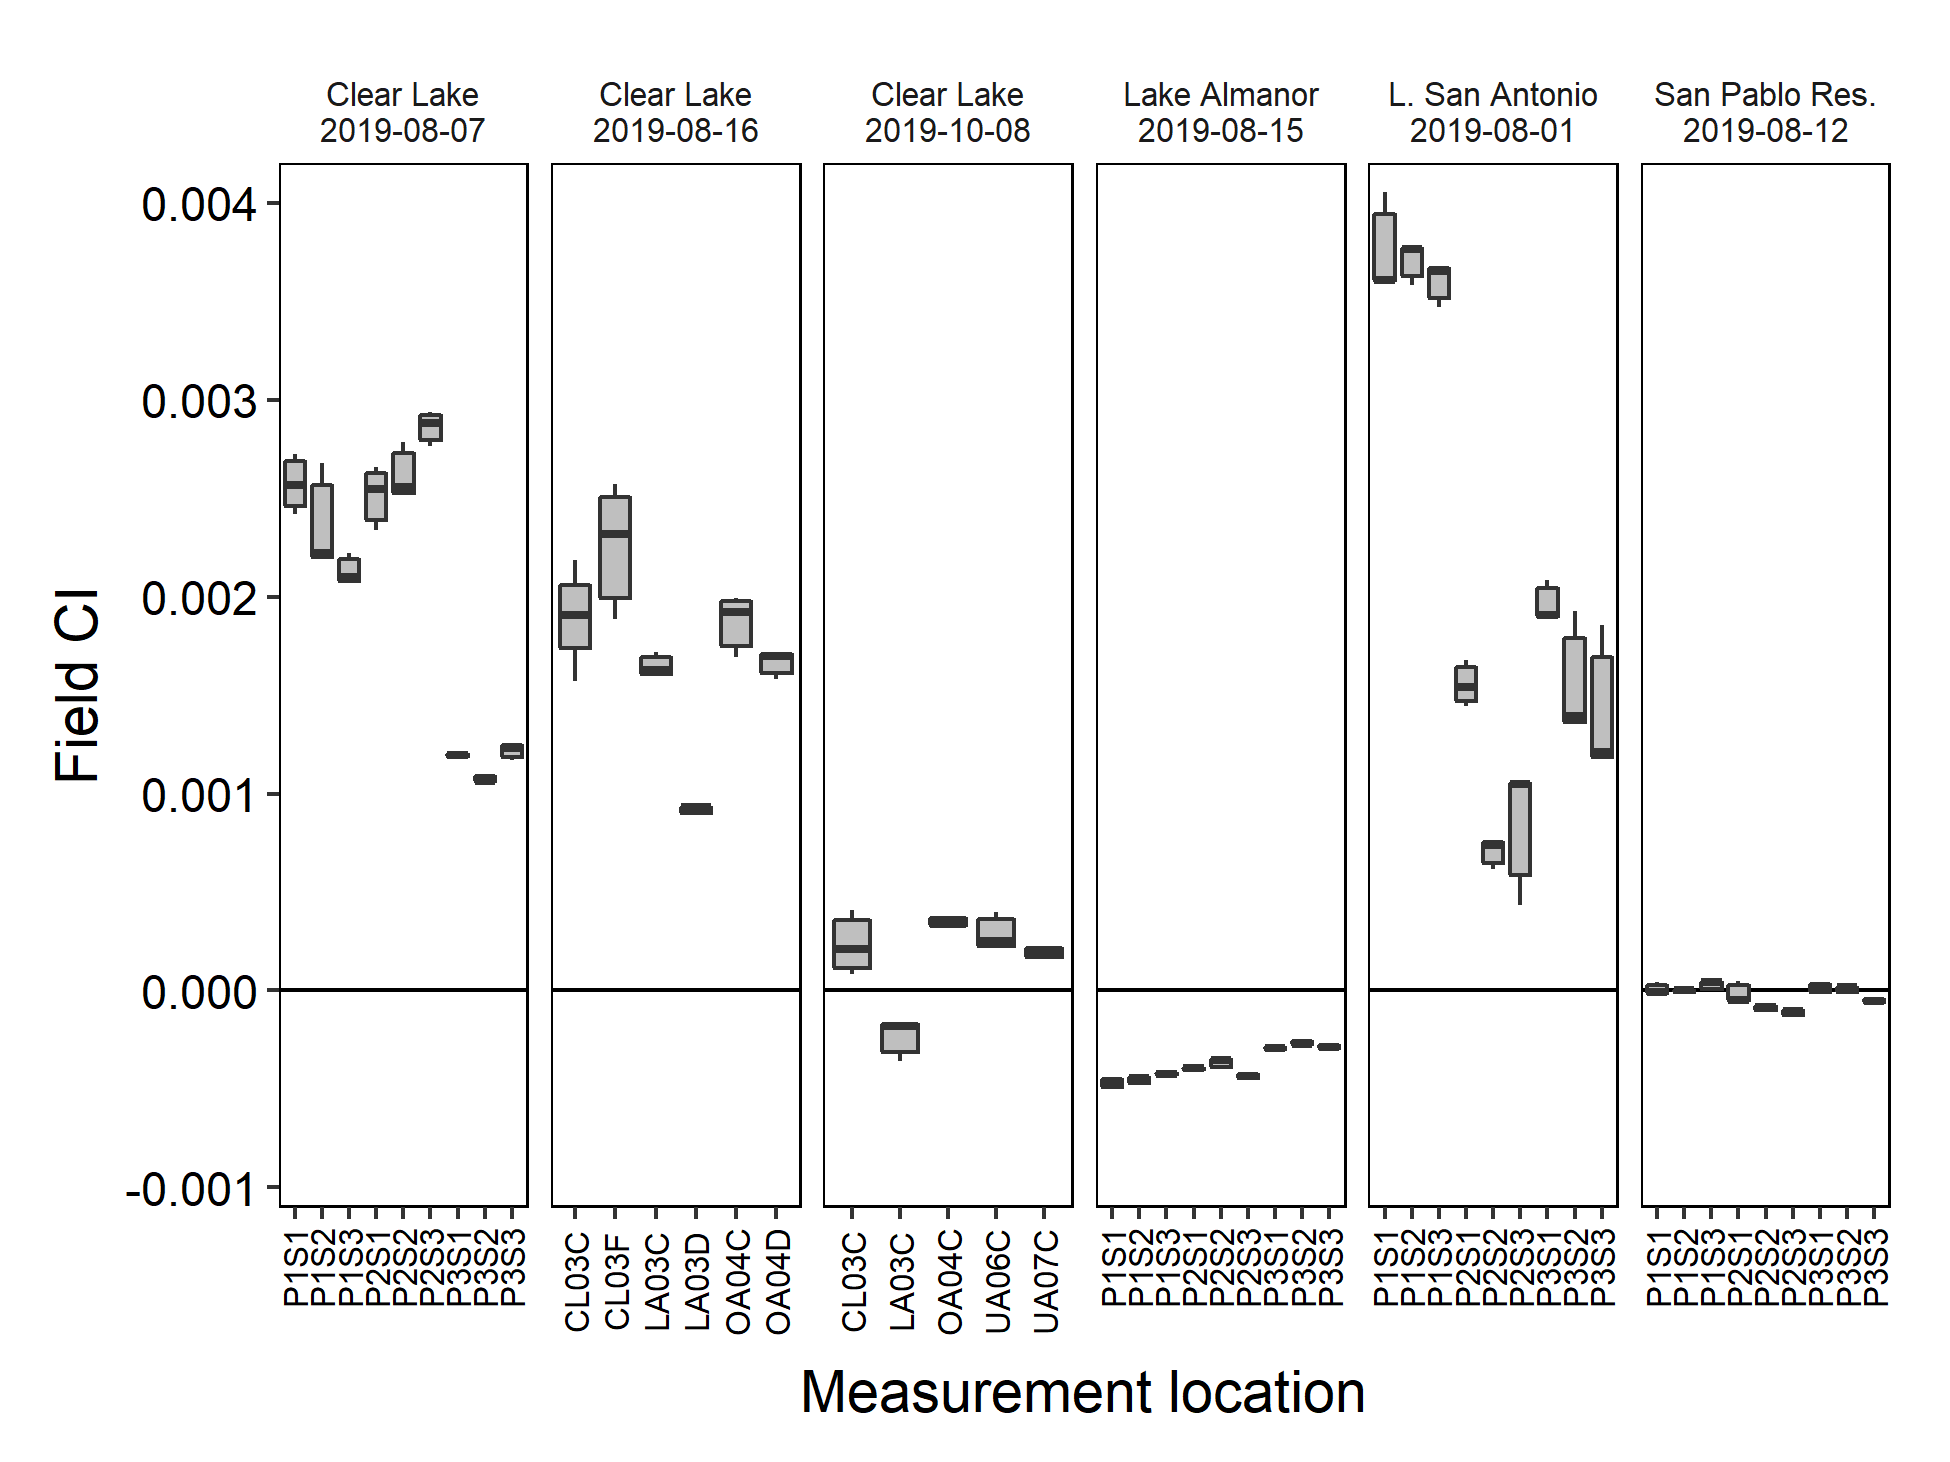
\includegraphics[width=0.6\linewidth]{../Data/Figures_output/ci_wbd} 

}

\end{figure}

\textbf{Figure 5.} CI values from all sampling locations.

The field data estimated higher cyanobacterial abundances than the
satellite data (Fig. 6). Both the satellite and field data estimated no
cyanobacteria at Lake Almanor and San Pablo Reservoir. The field and
satellite data were also well correlated in estimatinc cyanobacterial
abundances at Clear Lake on 07-Aug and a single pixel on
16-Aug.~However, all field data from Lake San Antonio, Clear Lake
08-Oct, and two pixels at Clear Lake 16-Aug suggested cyanobacterial
abundances, while the satellite estimated no cyanobacteria. The field CI
values correlated relatively better with chlorophyll-a levels (Fig. 7),
than with the the satellite CI values.

\begin{figure}

{\centering 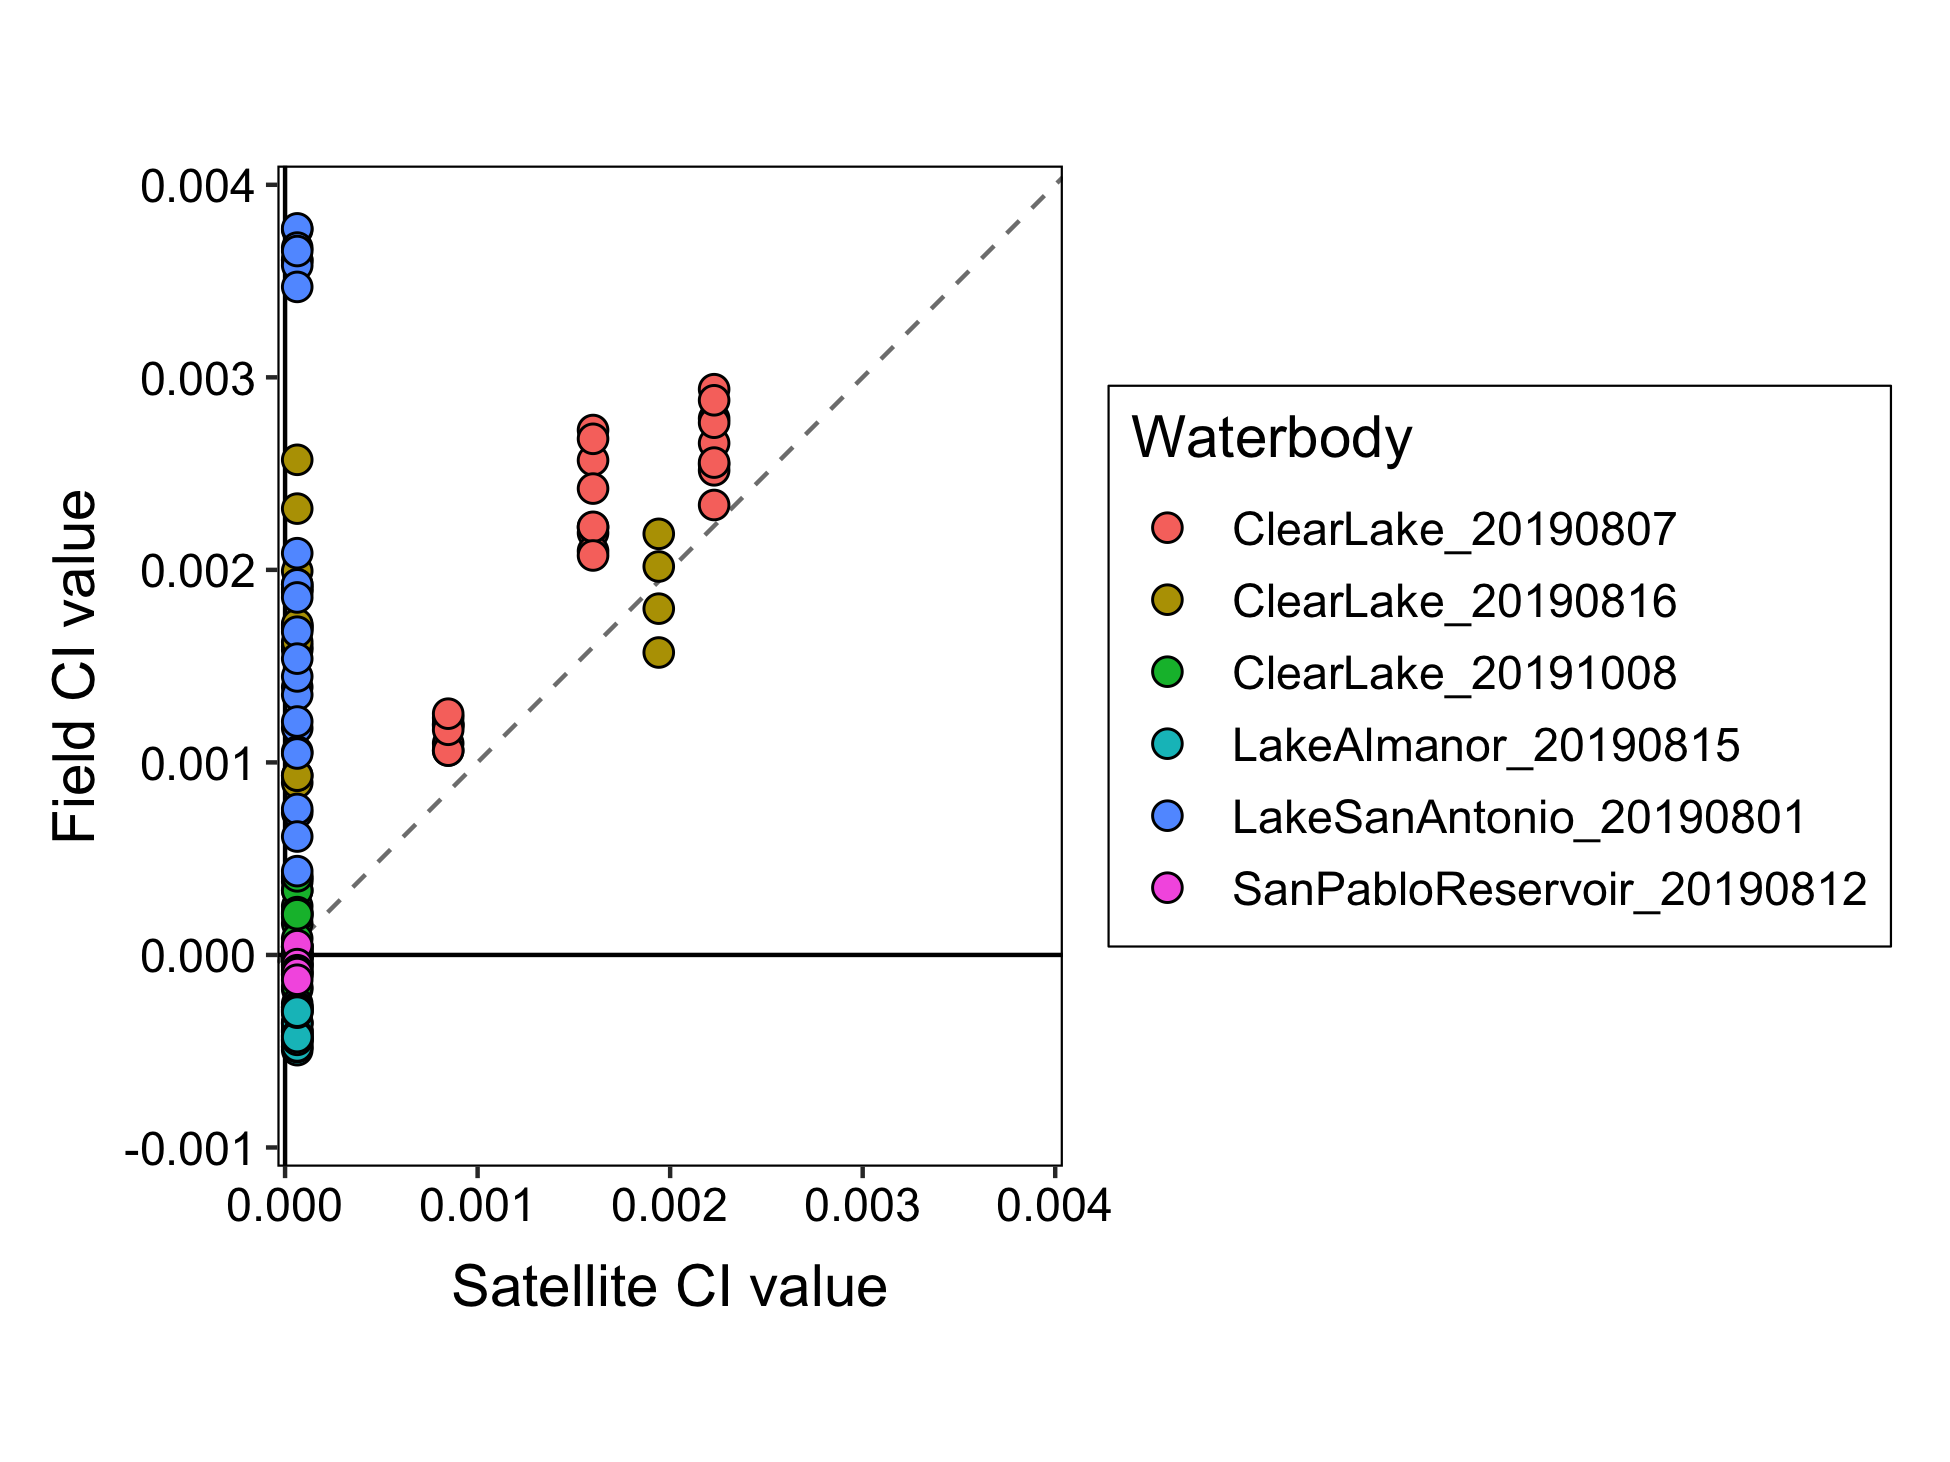
\includegraphics[width=0.6\linewidth]{../Data/Figures_output/ci_fs} 

}

\end{figure}
\begin{figure}

{\centering 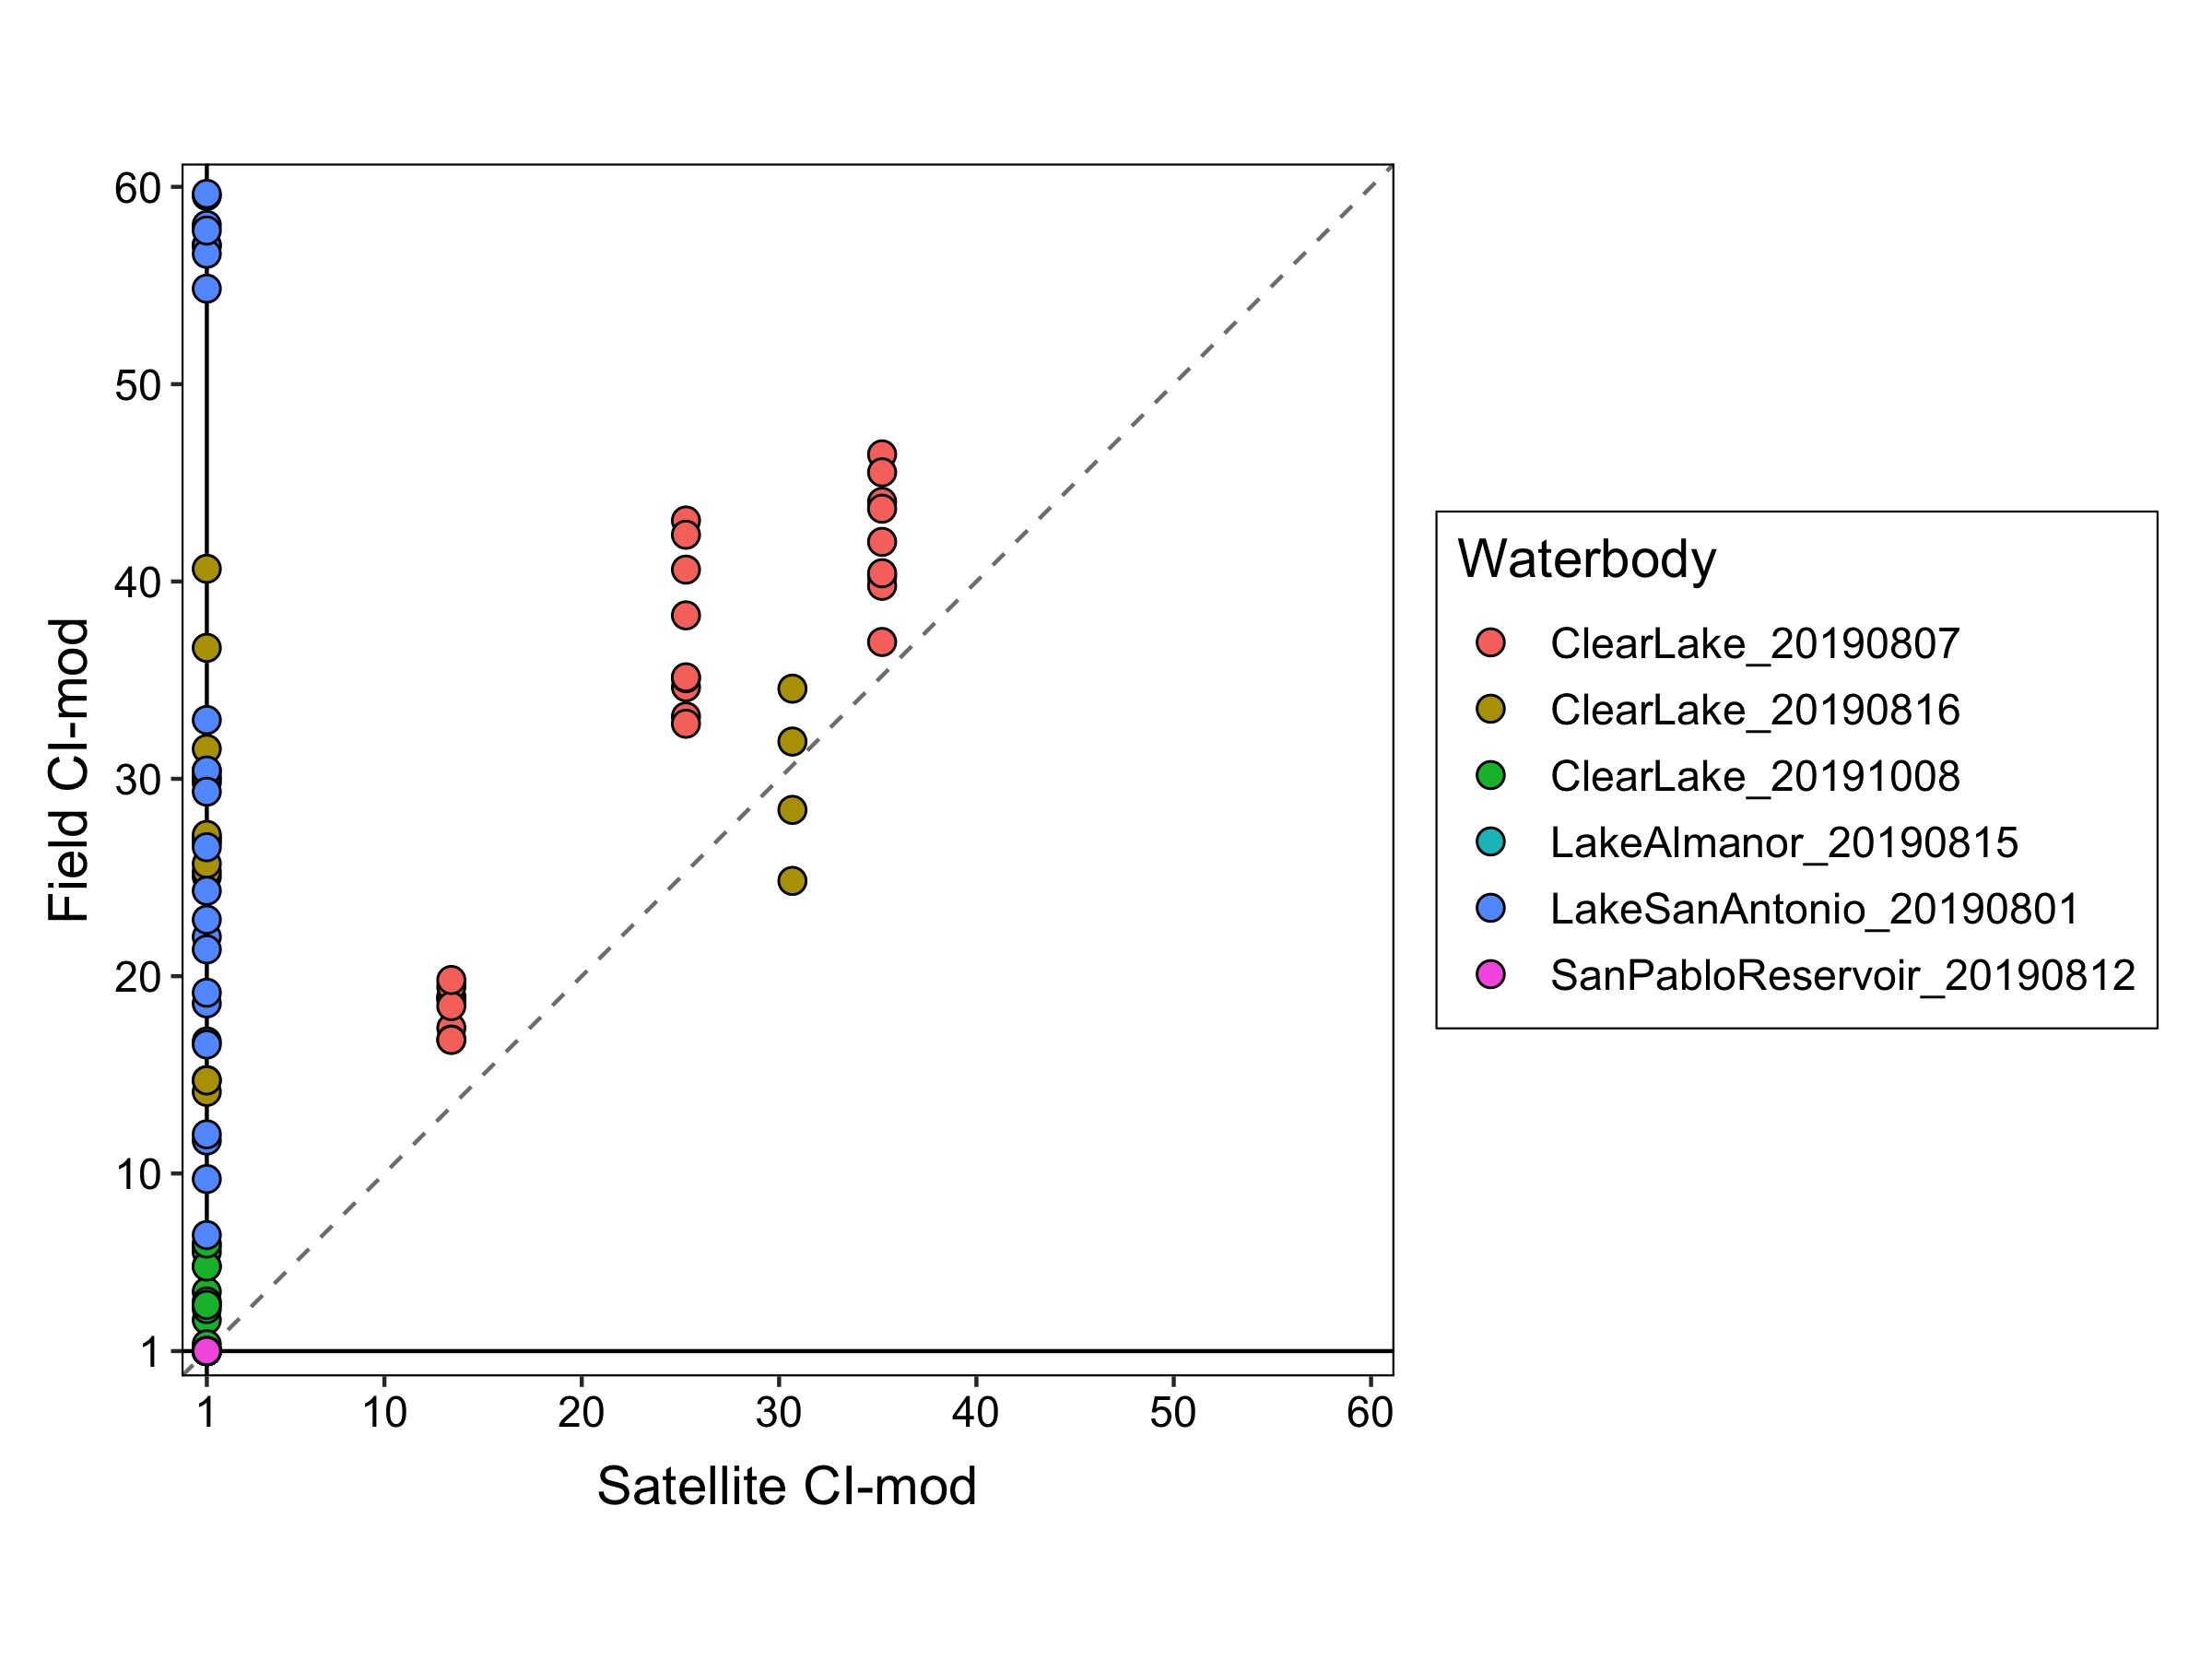
\includegraphics[width=0.6\linewidth]{../Data/Figures_output/ci_mod_fs} 

}

\end{figure}

\textbf{Figure 6.} Comparison of field and satellite data. Top panel)
Field CI values and Satellite CI values. Bottom panel) Field modified CI
values and satellite modified CI values (modified scale 1-1000. Colors
show the waterbody and sampling date. The 1:1 line is dashed.

\begin{figure}

{\centering 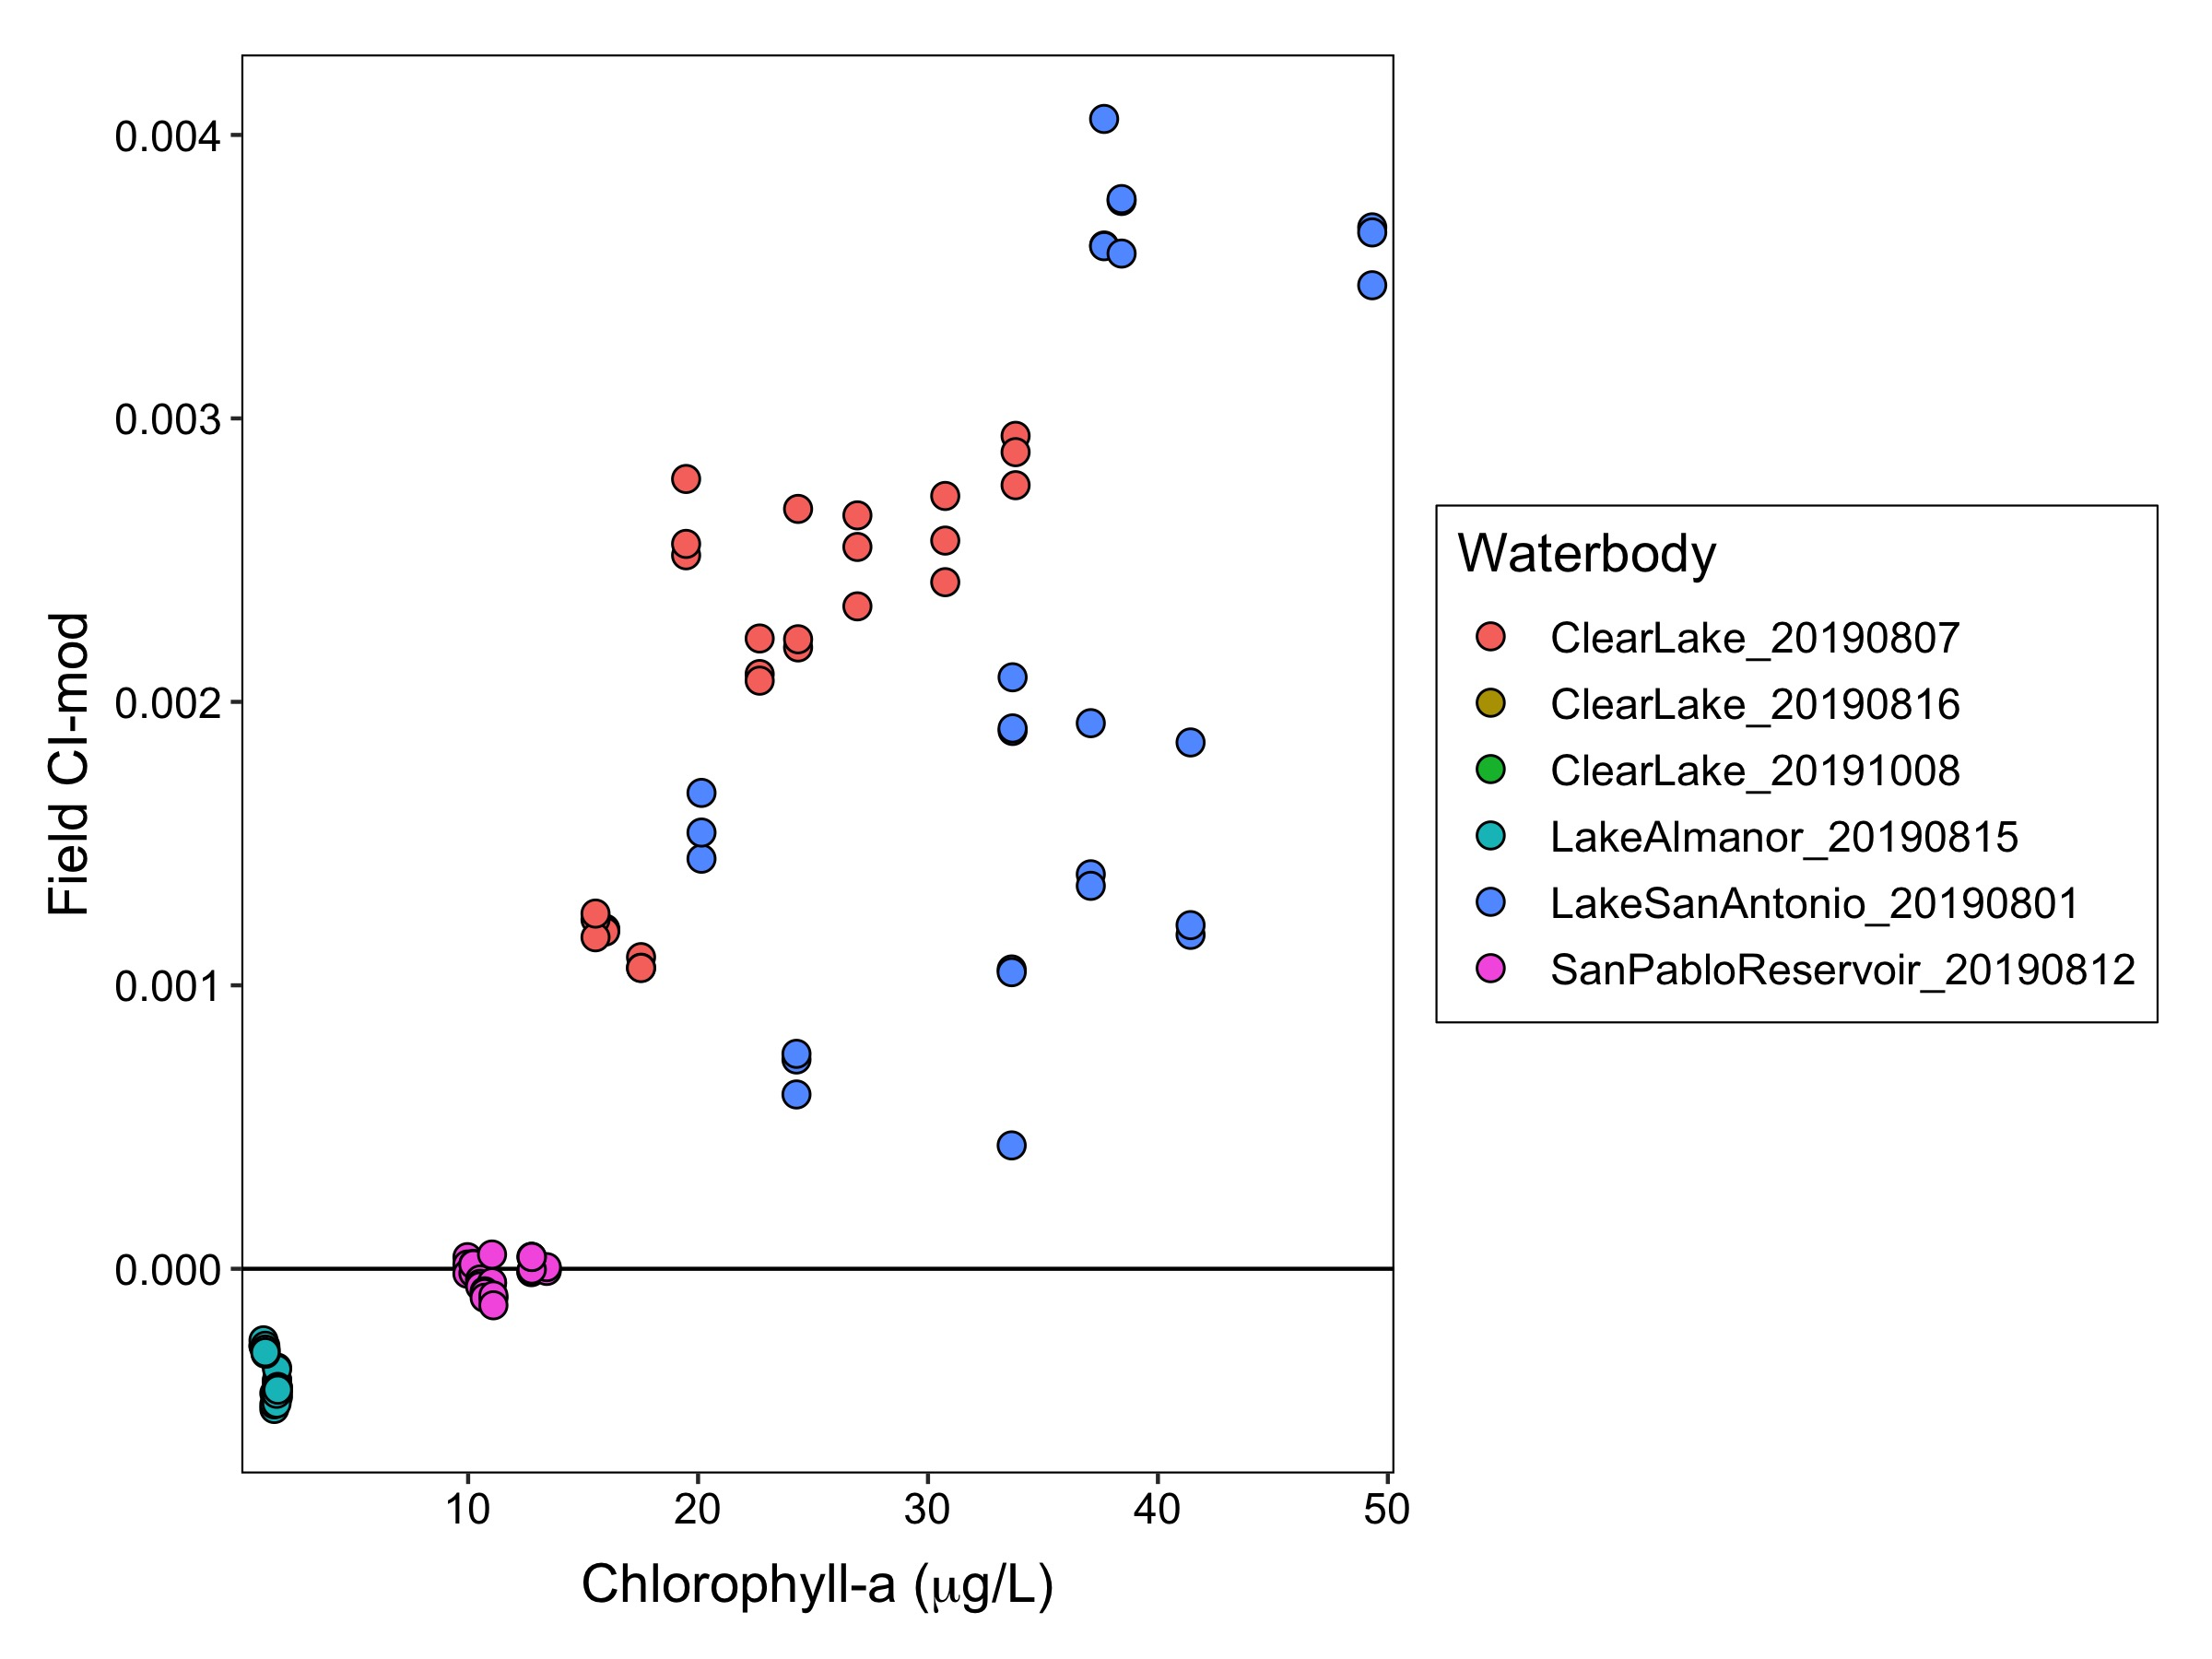
\includegraphics[width=0.6\linewidth]{../Data/Figures_output/ci_chla} 

}

\end{figure}

\textbf{Figure 7.} Comparison of field CI-mod and chlorophyll-a. Colors
show the waterbody and sampling date.

\hypertarget{discussion}{%
\subsection{\texorpdfstring{\textbf{Discussion}}{Discussion}}\label{discussion}}


\end{document}
